\documentclass[12pt, twoside]{article}
\usepackage[letterpaper, margin=1in, headsep=0.2in]{geometry}
\setlength{\headheight}{0.6in}
%\usepackage[english]{babel}
\usepackage[utf8]{inputenc}
\usepackage{microtype}
\usepackage{amsmath}
\usepackage{amssymb}
%\usepackage{amsfonts}
\usepackage{siunitx} %units in math. eg 20\milli\meter
\usepackage{yhmath} % for arcs, overparenth command
\usepackage{tikz} %graphics
\usetikzlibrary{quotes, angles}
\usepackage{graphicx} %consider setting \graphicspath{{images/}}
\usepackage{parskip} %no paragraph indent
\usepackage{enumitem}
\usepackage{multicol}
\usepackage{venndiagram}

\usepackage{fancyhdr}
\pagestyle{fancy}
\fancyhf{}
\renewcommand{\headrulewidth}{0pt} % disable the underline of the header
\raggedbottom
\hfuzz=2mm %suppresses overfull box warnings

\usepackage{hyperref}

\fancyhead[LE]{\thepage}
\fancyhead[RO]{\thepage \\ Name: \hspace{4cm} \,\\}
\fancyhead[LO]{BECA / Dr. Huson / Geometry\\*  Unit 6: Analytic geometry\\* 14 December 2022}

\begin{document}

\subsubsection*{6.5 PreQuiz: Slope-intercept form of linear equations \hfill 8.F.A.3}
\begin{enumerate}

\item Find the equation of the given line $\overleftrightarrow{AB}$, $A(0,2)$, $B(3,5)$.
\begin{multicols}{2}
    \begin{enumerate}[itemsep=0.5cm]
      \item Find the slope. \par
          $m=$
      \item Write down the $y$-intercept. \par 
        $b=$
      \item Write the equation of the line. \vspace{1cm}
      \end{enumerate}
    \begin{flushright}
    \begin{tikzpicture}[scale=0.8]
      \draw [help lines] (-1,-1) grid (6,6);
      \draw [thick, ->] (-1.2,0) -- (6.4,0) node [below right] {$x$};
      \draw [thick, ->] (0,-1.2)--(0,6.4) node [left] {$y$};
      \draw [fill] (0,2) circle [radius=0.05] node[below right] {$A(0,2)$};
      \draw [fill] (3,5) circle [radius=0.05] node[below right] {$B(3,5)$};
      \draw [<->, thick, domain=-1.2:4.2] plot (\x,\x+2);
    \end{tikzpicture}
    \end{flushright}
  \end{multicols}

\item Is the point $(4,7)$ on the line $y=3x-5$? Support your answer algebraically. \vspace{3cm}

\item Answer each statement about linear equations.
\begin{enumerate}[itemsep=0.25cm]
  \item What is the slope of a horizontal line?
  \item What is the $y$-intercept of the line $y = 2x + 3$?
  \item What is the slope of the line $y = x - 5$?
  \item Which has an undefined slope, a vertical or horizontal line?
  \item What is the $y$-intercept of the line $y = -2x$?
\end{enumerate} \vspace{0.5cm}

\item A line has a slope of $-\frac{3}{2}$ and passes through the point $(0, 2)$. Write down the equation of the line in the form $y=mx+b$. \vspace{3cm}

\newpage
\subsubsection*{HSG.GPE.B.5 The slope criteria for parallel and perpendicular lines}
\item The line $j$ has the equation $y=2x-3$.
  \begin{enumerate}
    \item What is the slope of the line $k$, given $k \parallel j$?
    \vspace{1cm}
    \item What is the slope of the line $l$, given $l \perp j$?
    \vspace{1cm}
  \end{enumerate}

\item The line $l$ has the equation $y=-\frac{3}{5}x+4$. To each line below, circle whether $l$ is parallel, perpendicular, or neither.
\begin{enumerate}
  \item parallel \quad perpendicular \quad neither \qquad $y=\frac{3}{5}x-2$
  \vspace{0.5cm}
  \item parallel \quad perpendicular \quad neither \qquad $y=\frac{5}{3}x+9$
  \vspace{0.5cm}
  \item parallel \quad perpendicular \quad neither \qquad $y=-\frac{3}{5}x+1$
  \vspace{0.5cm}
  \item parallel \quad perpendicular \quad neither \qquad $y=-\frac{5}{3}x-7$
  \vspace{0.5cm}
\end{enumerate}


\item Write the linear equation $6x+2y=4$ in the form $y=mx+c$. \vspace{4cm}

\item The line has the equation $y=-4x+11$. 
\begin{enumerate}
  \item Write down it's slope and $y$-intercept. \hspace{1cm} $m=$
  \hspace{2cm} $b=$
  \item Is the point $(3, 1)$ on the line? Justify your answer.
\end{enumerate}
\vspace{4cm}

\end{enumerate}
\end{document}